%++++++++++++++++++++++++++++++++++++++++s\\
\documentclass[letterpaper,12pt]{article}
\usepackage{tabularx} % extra features for tabular environment
\usepackage{amsmath}  % improve math presentation
\usepackage{graphicx} % takes care of graphic including machinery
\usepackage[margin=1in,letterpaper]{geometry} % decreases margins
\usepackage{cite} % takes care of citations
\usepackage[final]{hyperref} % adds hyper links inside the generated pdf file
\usepackage{caption}
\usepackage{float}
\usepackage{subcaption}
\usepackage{hyperref}
\hypersetup{
	colorlinks=true,       % false: boxed links; true: colored links
	linkcolor=blue,        % color of internal links
	citecolor=blue,        % color of links to bibliography
	filecolor=magenta,     % color of file links
	urlcolor=blue         
}
%++++++++++++++++++++++++++++++++++++++++


\begin{document}

\title{732A75 Advanced Data Mining laboratory 2 report}
\author{Yuki Washio (timwa902) and Nicolas Taba (nicta839)}
\date{\today}
\maketitle



\section{Introduction}

The aim of this laboratory exercise is to use assosciation analysis to describe clusters obtained from a mined dataset.

In this laboratory, we use the iris dataset. This dataset features 50 instances of each 3 classes of flowers (Iris Setosa, Iris Versicolor and Iris Virginica). Each of these data points has data pertaining to the sepal and petal length and width given in cm.

We will be using the seed value 10 whenever prompted. We also set the lower bound of minimum support to 0.2 throughout.


\section{Using assosciation analysis with optimal parameters}

In this section of the laboratory, we know the make up of this dataset and want to familiarize ourselves with the assosciation analysis tool of Weka. We begin by discretizing the dataset in 3 bins of data since continuous attributes cannot be processed by the software. We perform the simple Kmeans algorithm on the data like in the previous laboratory and crosstabulate the clusters with the class labels.

\begin{figure}[H]
\begin{subfigure}{.5\textwidth}
  \centering
  % include first image
  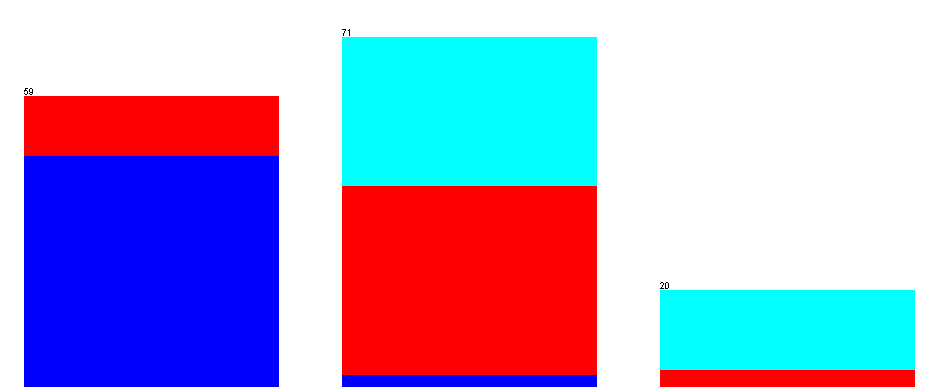
\includegraphics[width=.8\linewidth]{3bins_petalwidth}  
  \caption{data separated into 3 bins according to petalwidth}
  \label{fig:sub-first_1}
\end{subfigure}
\begin{subfigure}{.5\textwidth}
  \centering
  % include second image
  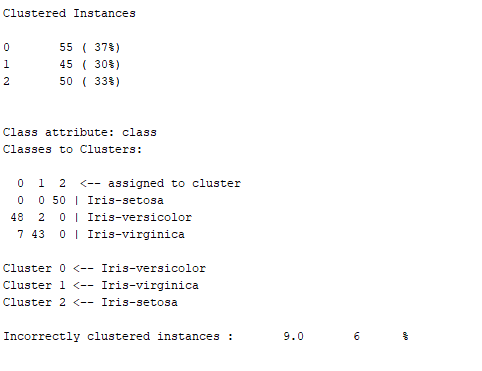
\includegraphics[width=.8\linewidth]{3bins_3cl_output}  
  \caption{kmeans clustering using k=3}
  \label{fig:sub-second_1}
\end{subfigure}
\caption{clustering using Kmeans with k=3 and n=3 bins}
\label{fig:fig_1}
\end{figure}

Here we see that a few elements of versicolor and virginica are wrongly clustered and account for a 68\% error in the clustering. We now perform the apriori algorithm on this clustering to try and ascertain if the rules used to make this clusters have high confidence.

We use the apriori algorithm to find rules that have the clusters as consequent.

\begin{figure}[H] 
  \centering
      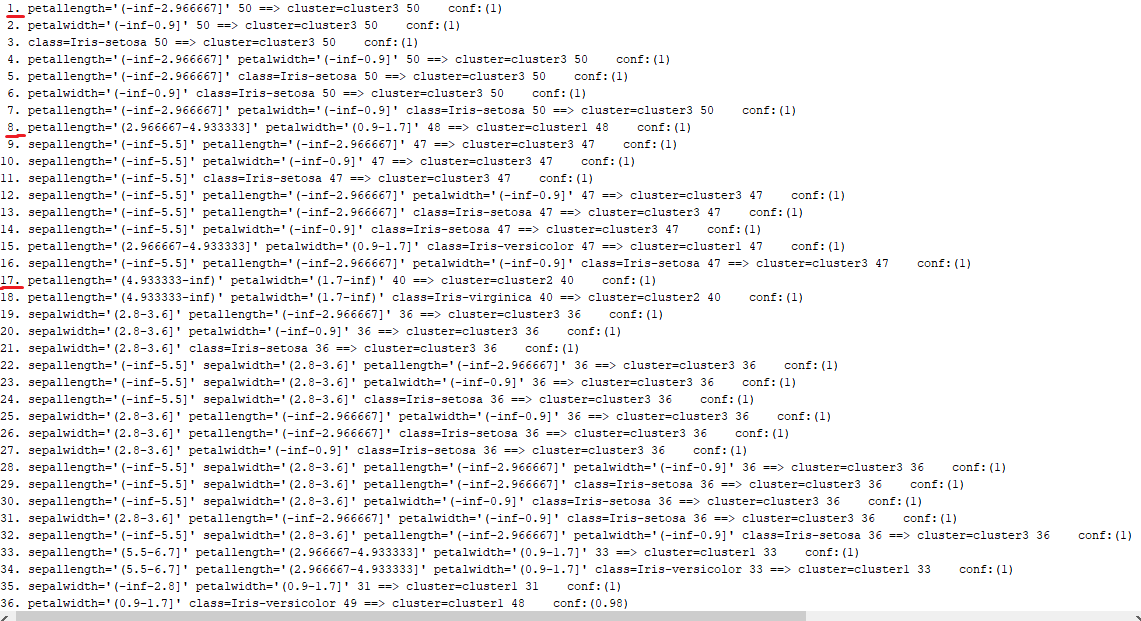
\includegraphics[width=0.8\columnwidth]{3_bins_3cl_apriori_rules}
        \caption{
                \label{fig:3bins_3cl_apriori}  
                Apriori rules for k=3 and n=3 bins.
        }
\end{figure}

In Fig.~\ref{fig:3bins_3cl_apriori}, we have the 36 best rules for this clustering solution. All 35 first rules point to all three clusters with a confidence of 100\%, with most rules indicating high confidence in identifying cluster 3 and few rules for clusters 2 and 1. The three best rules concern the petal length  for the Third cluster that is completely correctly identified (rule 1). The other rules that allow us to identify clusters 1 and 2 concern petal length and width and allow a good clustering as the support for these rules is the same than for the classes we clustered earlier in ig.~\ref{fig:sub-second_1}.

This is a good indication that our clustering is correct as several rules can be found to cluster the data to one class using one or many determinant with very high support. The 5 first rules in Fig.~\ref{fig:3bins_3cl_apriori} concern cluster 3 with a support of 50. This indicates that cluster 3 is the setosa class and that this particular class can easily be identified with respect to the others.

The documentation of the dataset indicates that one of the classes is linearly separable from the others whereas the other two are not linearly separable from each other. The result we obtained is thus the expected optimal parameters when we use a very well known dataset. (documentation: \url{https://www.ida.liu.se/~732A75/lab/iris.arff})

\section{Investigation of change of bins and cluster numbers}

We now wish to investigate how the change in number of bins and clusters affects the clustering algorithm and the apriori algorithm. We know from the previous laboratory that the assignment of the correct number of clusters to the number of classes that we believe compose the set is an important factor in how the Kmeans algorithm performs, but we do not know yet how the number of bins affects this performance. We will use the same process as previously with the apriori algorithm to assess these effects.

\subsection{Changing the number of bins}

We will keep the number of clusters fixed to the optimal value while changing the number of bins. We will use the previous result with n=3 and repeat the experiment with n=5 and 10.

\begin{figure}[H]
\begin{subfigure}{.5\textwidth}
  \centering
  % include first image
  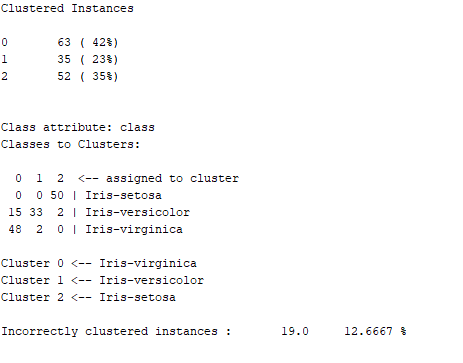
\includegraphics[width=.8\linewidth]{5bins_3cl_output}  
  \caption{Kmeans with 5 bins and k=3}
  \label{fig:sub-first_2}
\end{subfigure}
\begin{subfigure}{.5\textwidth}
  \centering
  % include second image
  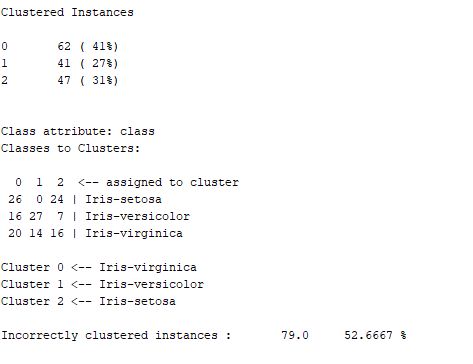
\includegraphics[width=.8\linewidth]{10_bins_3cl_output}  
  \caption{Kmeans with 10 bins and k=3}
  \label{fig:sub-second_2}
\end{subfigure}
\begin{subfigure}{.5\textwidth}
  \centering
  % include second image
  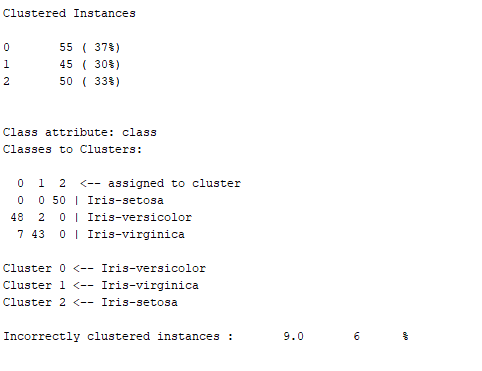
\includegraphics[width=.8\linewidth]{3bins_3cl_output}  
  \caption{Kmeans with 3 bins and k=3}
  \label{fig:sub-third_2}
\end{subfigure}
\caption{Kmeans algorithm output using different number of bins}
\label{fig:fig_2}
\end{figure}

From Fig.~\ref{fig:fig_2}, we can see that increasing the number of bins has decreased the performance of the Kmeans algorithm. When the number of bins is much larger than the optimal (n=10 bins) we find that the performance goes as low as 52\% error rate in this case. Most of the errors occur for the versicolor and virginica in the case of n= 5.

We now try to find rules assosciated to each clusters for 5 and 10 bins.

\begin{figure}[H] 
  \centering
      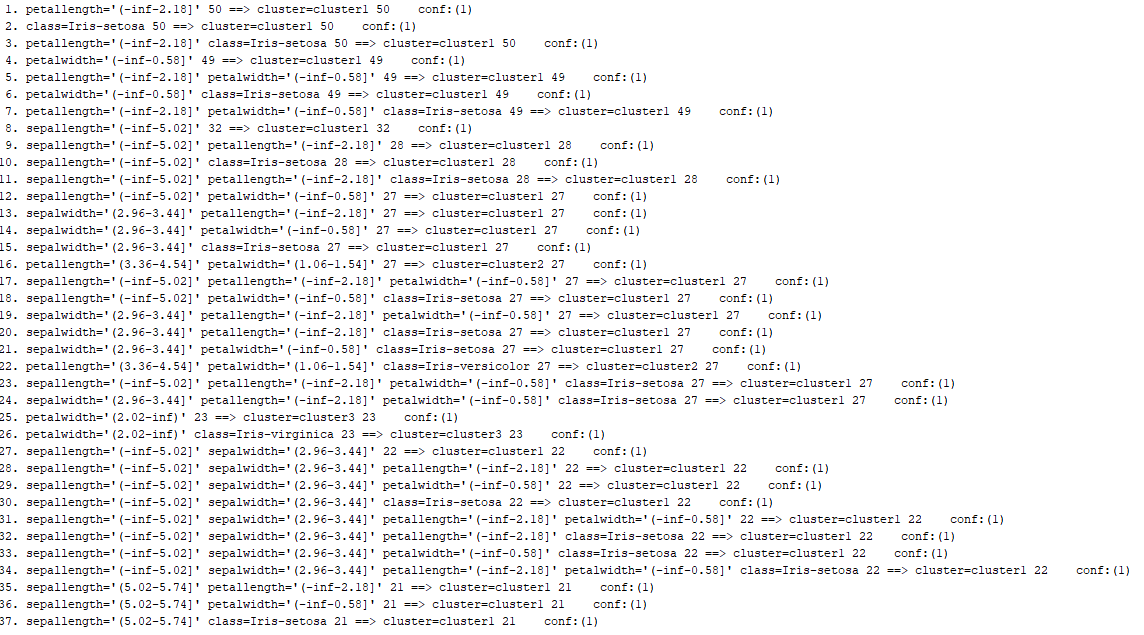
\includegraphics[width=0.8\columnwidth]{5_bins_3cl_apriori_rules}
        \caption{
                \label{fig:5bins_3cl_apriori}  
                Apriori rules for k=3 and n=5 bins.
        }
\end{figure}


\begin{figure}[H] 
  \centering
      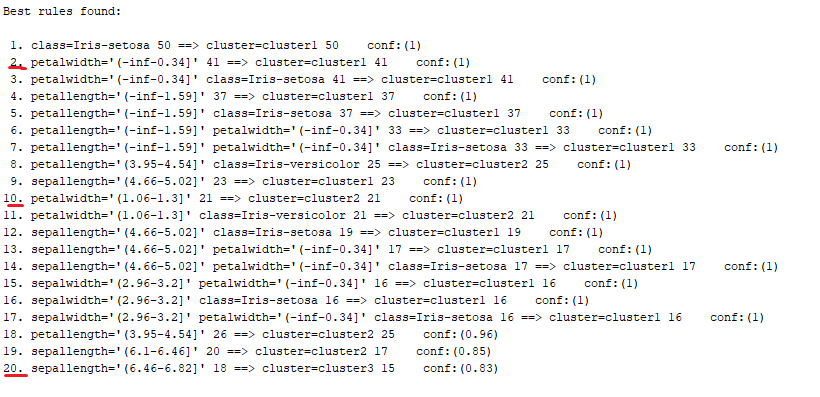
\includegraphics[width=0.8\columnwidth]{10_bins_3cl_apriori_rules}
        \caption{
                \label{fig:10bins_3cl_apriori}  
                Apriori rules for k=3 and n=10 bins.
        }
\end{figure}

In Fig.~\ref{fig:5bins_3cl_apriori} we see that the rules with highest confidence mostly point to cluster 1. There are some instances of cluster 3 being a consequent (rule 26 and 27). We can think from this that only 1 class can be clearly said to be dissimilar to the others. The best rules for clustering are marked in red.

In Fig~\ref{fig:10bins_3cl_apriori}, we find only 20 rules with high confidence ($>0.8$) with rules that have all 3 clusters as consequent. However, we will notice that some of these rules are not "good" rules such as rule 1 that has "belonging to class iris-setosa" yielding cluster 1. This is not a good rule. We can ascertain from these rules that the bin number is not the correct one since the rules that we get are not good with some having low support 15 instances for rule 20 for example. The best rules are marked in red.

When we change the number of bins, we move the intervals that were used to differentiate when we only had 3 bins. With different intervals, we also notice that there are some instances where some clusters do not have enough minimum support. For exmaple, in the case of cluster 1, using 5 bins, we have a support of 35/150 which is smaller than the required 0.2. This is why although the confidence in the rules is high, the support is very low and we do not trust these rules.

\subsection{Changing the number of clusters}

We now will investigate how the number of clusters affects the clustering algorithm and how the effects identified in the previous lab can be also identified using the rules produced by the apriori algorithm.

We will keep n=3 bins constant while varying the number of clusters that are investigated.


\begin{figure}[H]
\begin{subfigure}{.5\textwidth}
  \centering
  % include first image
  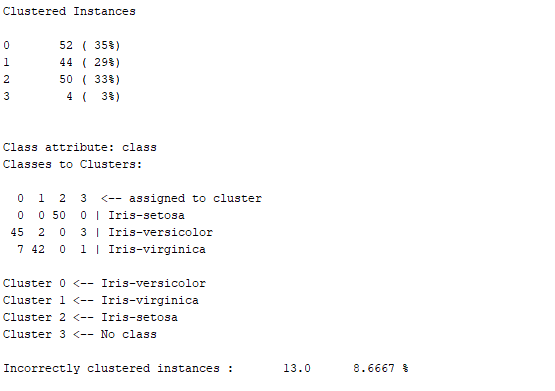
\includegraphics[width=.8\linewidth]{3bins_4cl_output}  
  \caption{Kmeans with 3 bins and k=4}
  \label{fig:sub-first_3}
\end{subfigure}
\begin{subfigure}{.5\textwidth}
  \centering
  % include second image
  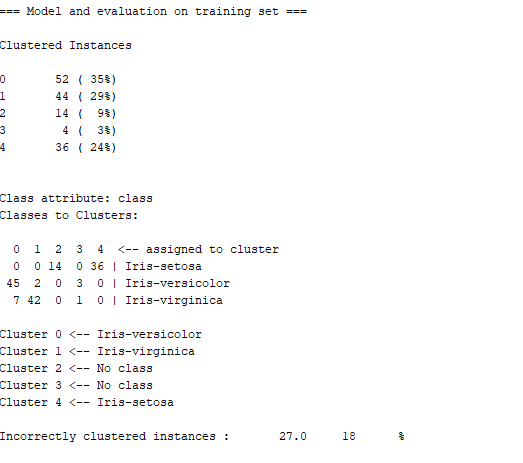
\includegraphics[width=.8\linewidth]{3bins_5cl_output}  
  \caption{Kmeans with 3 bins and k=5}
  \label{fig:sub-second_3}
\end{subfigure}
\caption{Kmeans algorithm output using different number of clusters and the same number of bins}
\label{fig:fig_3}
\end{figure}

In Fig~\ref{fig:fig_3}, we observe that the number of incorrectly clustered instances increases with a rate going from 6\% in the optimal case to 18\% for 5 clusters. In the case of 4 clusters, all instances of setosa are correctly identified and cluster 3 has very few elements. This could lead us to think already at this point that some of these elements could be clustered elsewhere or are maybe a group of outliers belonging to another class. 

We now investigate the rules that are yielded by the apriori algorithm for the previous two cases.


\begin{figure}[H] 
  \centering
      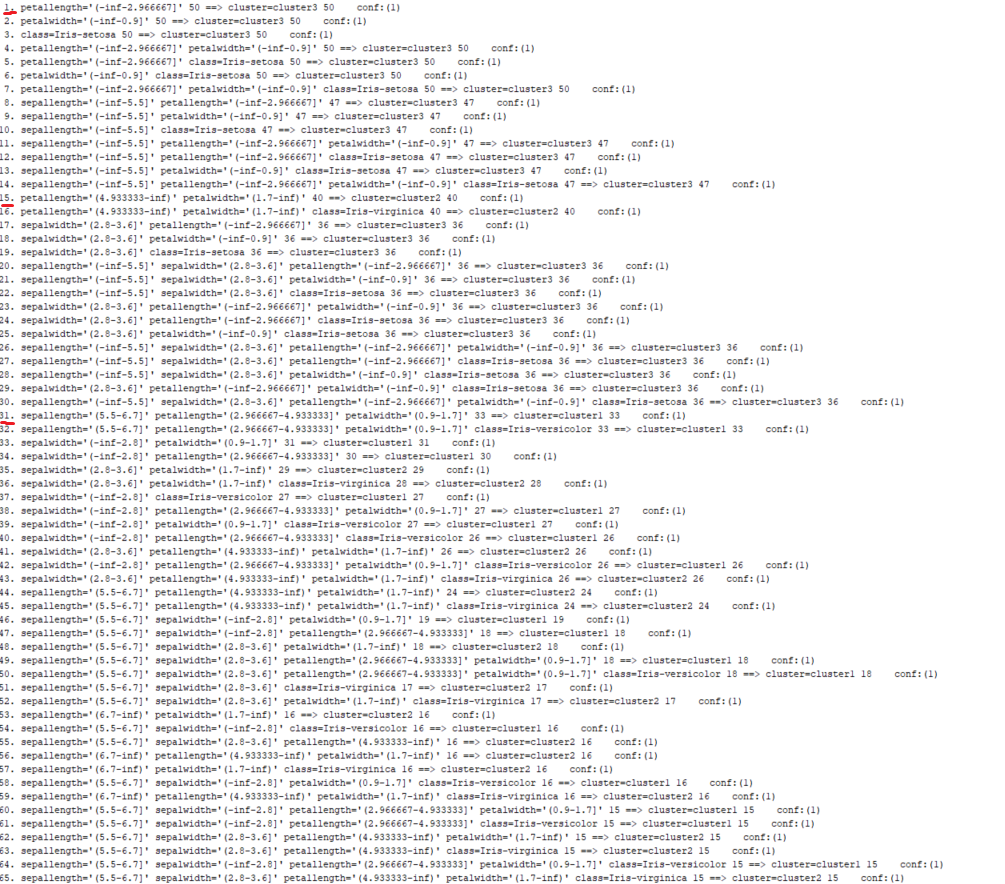
\includegraphics[width=0.8\columnwidth]{3bins_4cl_apriori_rules}
        \caption{
                \label{fig:3bins_4cl_apriori}  
                Apriori rules for k=4 and n=3 bins.
        }
\end{figure}


\begin{figure}[H] 
  \centering
      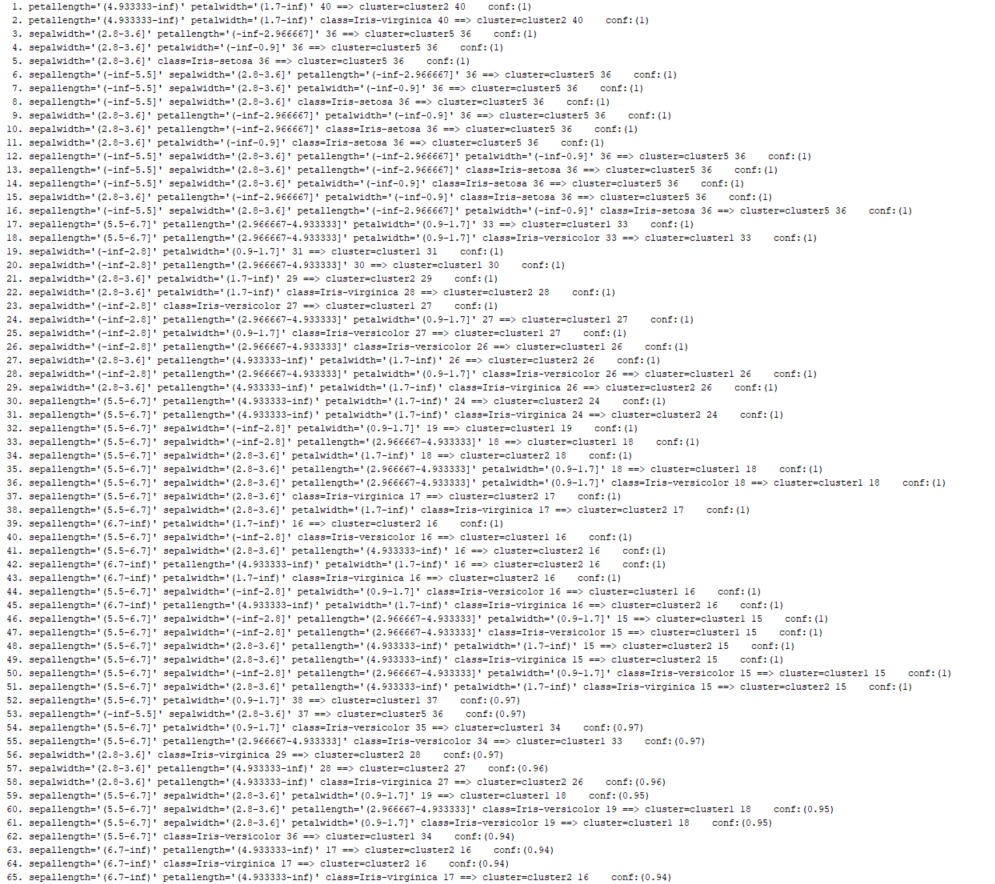
\includegraphics[width=0.8\columnwidth]{3bins_5cl_apriori_rules}
        \caption{
                \label{fig:3bins_5cl_apriori}  
                Apriori rules for k=5 and n=3 bins.
        }
\end{figure}

As stated in the previous section, the rules produced here are not good rules. They contain determinants that have the class attribute to establish a rule to a cluster consequent. Although they have high confidence, the support for some of these rules is low with many values below 20. Due to these rules being of poor quality, we are lead to think that the clustering is erroneous. The best rules for each clustering are marked in red. Moreover, we will note here that among the best rules, we do not find rules for some clusters. In Fig~\ref{fig:3bins_4cl_apriori}, we do not find rules for the 4th cluster that have high confidence since the clsuter only contains 4 individuals. In \ref{fig:3bins_5cl_apriori}, similarly, we do not find rules for the thrid and fourth clusters.

When we increase the number of clusters, we find clusters with a very small number of cases. This makes it impossible for some cluster elements to have the required minimum support to establish rules for them using assosication analysis.


\section{Discussion}

In this work, we established that the apriori algorithm could be used to ascertain the quality of a clustering algorithm by analyzing the rules it yields. A primary glance at the Kmeans algorithm can indicate if there are issues in the number of bins or clusters. Too many clusters or bins will yield poor performance and many errors of clustering.


\end{document}
